\renewcommand{\figurename}{Rys.}

\chapter{Sprzętowa realizacja układu pomiarowego}
\label{cha:Sprzęt}

\fontsize{14}{15}\selectfont

%---------------------------------------------------------------------------
Optyczna metoda wyznaczania nasycenia krwi tętniczej tlenem oraz tętna bazuje na analizie krzywej pletyzmograficznej, uzyskanej w~procesie transluminacji tkanek przy zastosowaniu dwóch długości fali.
Odpowiednimi źródłami fal elektromagnetycznych w~zakresie promieniowania widzialnego i~bliskiej podczerwieni są ogólnodostępne diody elektroluminescencyjne, emitujące promieniowanie w~wąskim 
zakresie częstotliwości. Detekcja sygnału użytecznego w~procesie prześwietlania odbywa się przy pomocy fotodiody, która pracując jako źródło prądowe, generuje prąd wprost proporcjonalny do 
padającego promieniowania. Fotoprąd niosący użyteczną informację dla procesu pulsoksymetrii, trafia do układów konwersji, gdzie zostaje zamieniony na łatwiejszy w~użyciu sygnał napięciowy. Dalej 
przeprowadzany jest proces filtracji oraz kondycjonowania, aby ostatecznie poprzez przetwornik analogowo~-~cyfrowy sygnał napięciowy mógł być wykorzystany przez system mikroprocesorowy 
w~celu wyznaczenia poszukiwanych parametrów i~wskaźników.

Schemat komercyjnego aparatu pomiarowego przedstawia rysunek~\ref{rys:Schematic}. Nowoczesne rozwiązania w~postaci rozbudowanych układów wbudowanych dostarczają szerokiej funkcjonalności 
zapewniając wygodę użytkowania. Zasilanie bateryjne, wyświetlacze LCD, panele dotykowe oraz łatwy w~użyciu interfejs~użytkownika umożliwiają przeprowadzanie pomiarów przez pacjenta w~dowolnym 
miejscu bez pomocy operatora.
\begin{figure}[!h]
	\centerline{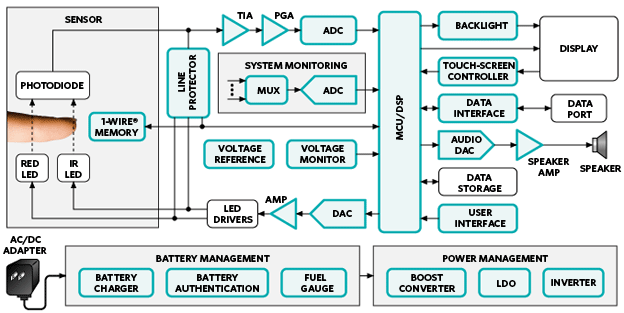
\includegraphics[scale = 0.76]{graphic/Schematic}}
	\caption{Schemat blokowy komercyjnego aparatu pomiarowego}
	~\\
	(źródło: http://www.maximintegrated.com)
	\label{rys:Schematic}
\end{figure}

W~niniejszej pracy zrealizowane zostaną elementy układu, niezbędne do wykonania pomiarów szukanych parametrów częstości akcji serca i~saturacji. Zakres prac wykonywanych przez autora projektu
zawiera schemat na rysunku~\ref{rys:MySchematic}.
\begin{figure}[!h]
	\centerline{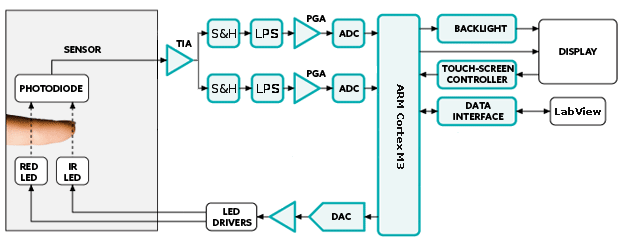
\includegraphics[scale = 0.76]{graphic/MySchematic}}
	\caption{Schemat blokowy pulsoksymetru wykonywanego w~ramach pracy}
	~\\
	(źródło: http://www.maximintegrated.com)
	\label{rys:MySchematic}
\end{figure}


\section{Układ sterowania natężeniem promieniowania LED}
\label{sec:LedSterownik}

Źródła światła w~postaci diod elektroluminescencyjnych generują promieniowanie, którego natężenie jest wprost proporcjonalne do prądu przepływającego przez obszar aktywny złącza P-N~(rys.~\ref{rys:LED}).
Najprostszym sposobem regulacji natężenia promieniowania jest szeregowe połączenie diody z~układem źródła prądowego sterowanego napięciowo, umożliwiającego liniową regulację przepływającego prądu. Możliwość 
płynnej regulacji intensywności światła umożliwia dostosowanie punktu pracy diody do grubości i~struktury badanego obiektu oraz umożliwia kompensowanie nierównomiernej charakterystyki czułości fotodiody~(rys.~\ref{rys:BPW34}).
\begin{figure}[!ht]
	\centerline{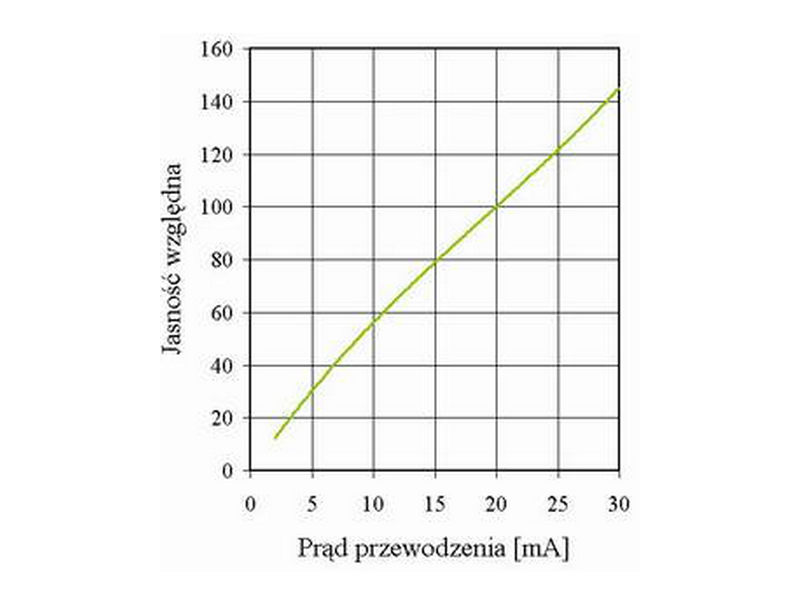
\includegraphics[scale = 0.46]{graphic/LED}}
	\caption{Zależność względnego natężenia promieniowania diody od przepływającego prądu przewodzenia}
	~\\
	(źródło: http://www.lediko.com)
	\label{rys:LED}
\end{figure}

\begin{figure}[!ht]
	\centerline{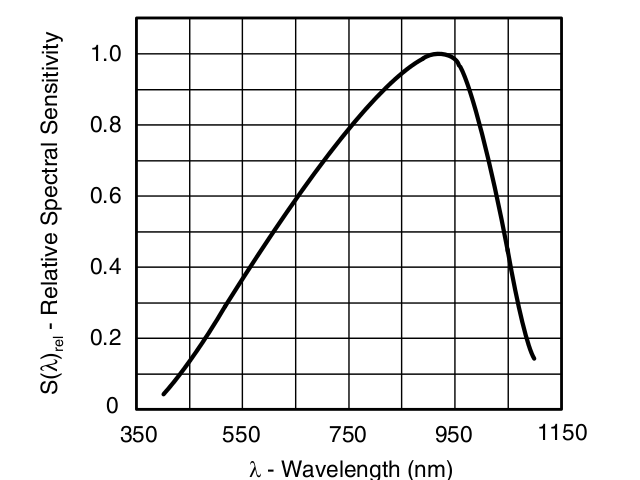
\includegraphics[scale = 0.46]{graphic/BPW34}}
	\caption{Względna charakterystyka czułości fotodiody PIN typu BPW34}
	~\\
	(źródło: na podstawie \cite{BPW34})
	\label{rys:BPW34}
\end{figure}

Przykład sterowanego źródła prądowego wykorzystanego w~projekcie pulsoksymetru przedstawiono na rysunku~\ref{rys:Led_Control}a. Zastosowanie wzmacniacza operacyjnego powoduje zwiększenie impedancji
wejściowej, co skutecznie zmniejsza obciążenie źródła sygnału sterującego. Pętla ujemnego sprzężenia zwrotnego obejmująca złącze emiter-baza tranzystora bipolarnego umożliwia liniową regulację
prądu wyjściowego przy pomocy napięcia sterującego. Duże wzmocnienie wzmacniacza operacyjnego oraz istnienie pętli ujemnego sprzężenia zwrotnego powodują powstanie masy pozornej pomiędzy wejściami wzmacniacza. 
Przy założeniu równych potencjałów na obu wejściach wzmacniacza uzyskujemy następujące równanie napięciowego prawa Kirchoffa: 
\begin{equation}
\label{equ:Kirchoff1}
	V_{IN} - V_{R_{1}} = 0,	
\end{equation}
gdzie:\\
$V_{R_{1}} = IR_{1}$

\begin{equation}
\label{equ:Kirchoff2}
	I = \frac{V_{IN}}{R_{1}}
\end{equation}

Metoda pomiarowa zakłada detekcję natężenia promieniowania pochodzącego od dwóch źródeł promieniowania, przy czym niedozwolona jest sytuacja równoczesnego zasilania źródeł światła w~określonej chwili czasowej.
W~tym celu równolegle do diody elektroluminescencyjnej dodano tranzystor polowy MOSFET z~kanałem typu~P stanowiący prosty układ kluczujący~(rys:~\ref{rys:Led_Control}b).
\begin{figure}[ht]
	\centerline{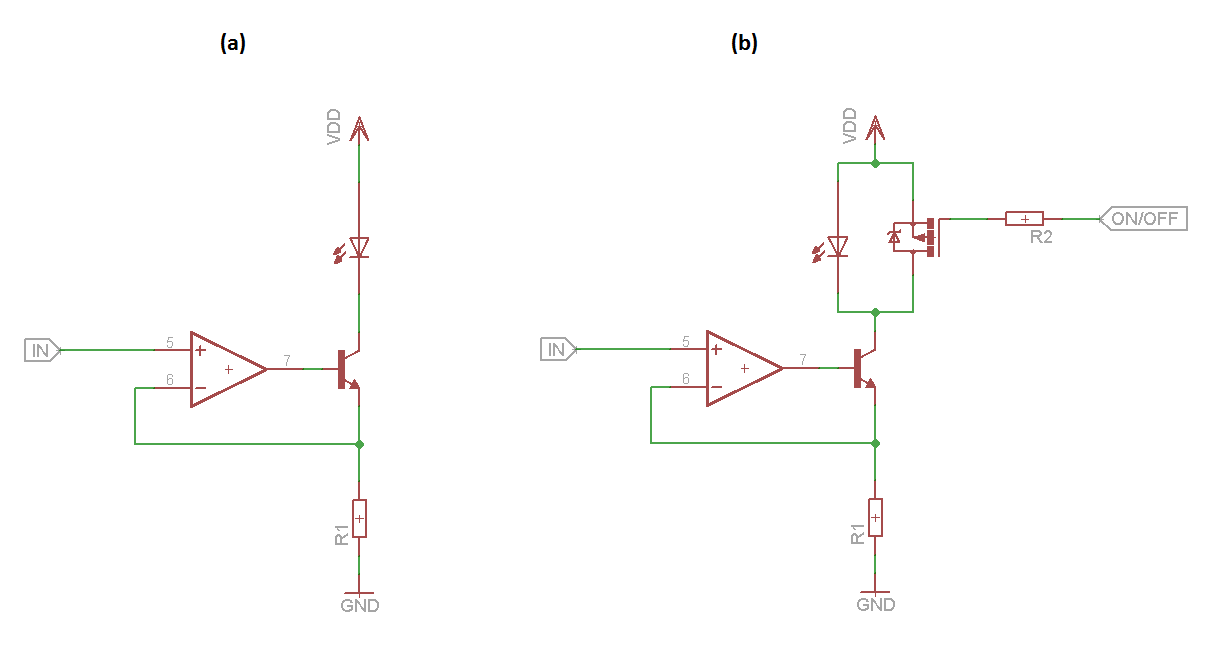
\includegraphics[scale = 0.58]{graphic/Led_Control}}
	\caption{Dioda LED zasilana źródłem prądowym sterowanym napięciowo}
	~\\
	(źródło: Schemat PCB)
	\label{rys:Led_Control}
\end{figure}

Sterując odpowiednio napięciem bramki, tranzystor polowy wprowadzany jest w~stan całkowitego otwarcia lub w~stan zatkania. W~stanie otwarcia cały prąd źródła płynie przez otwarty kanał tranzystora 
uniemożliwiając zasilenie diody. Tranzystory stanowiące przełączane klucze uruchamiane są naprzemiennie z~częstotliwością 1~kHz. 

Zakres liniowej regulacji prądu napięciem sterującym $V_{IN}$ ograniczony jest stanem nasycenia tranzystora bipolarnego. Wartość maksymalnego napięcia sterującego, dla którego tranzystor 
znajduje się w~stanie nasycenia wynosi:
\begin{equation}
\label{equ:Saturation1}
	V_{IN_{max}} = V_{DD} - V_{D} - V_{CES}
\end{equation}
gdzie:\\
$V_{CES}$ - napięcie nasycenia złącza emiter-kolektor,\\
$V_{D}$ - napięcie na diodzie elektroluminescencyjnej. 

\subsubsection{Sonda pomiarowa pulsoksymetru}
\label{subsubsec:Sonda}

Proces prześwietlania tkanek żywych metodą transluminacji, dokonywany jest poprzez poddanie promieniowaniu silnie ukrwionych i~stosunkowo cienkich fragmentów ciała, takich jak końcówki palców oraz 
płatki uszu. W~niniejszej pracy skupiono się na wariancie prześwietlania palców w~miejscach występowania płytek paznokci. W~celu zapewnienia odpowiednich warunków pomiaru oraz komfortu badanej osoby 
zastosowano dedykowaną sondę pomiarową w~formie zaciskanego klipsa umieszczanego na palcach~(rys:~\ref{rys:Sonda}).
Sonda wyposażona jest w~diody LED emitujące promieniowanie w~zakresie 660~nm i~940~nm oraz fotodiodę PIN, której charakterystyka czułości obejmuje obie długości fali. Przewód łączący sondę z~urządzeniem
pomiarowym zawiera ekran minimalizujący wpływ zakłóceń zewnętrznych na użyteczny sygnał prądowy fotodiody.
\begin{figure}[ht]
	\centerline{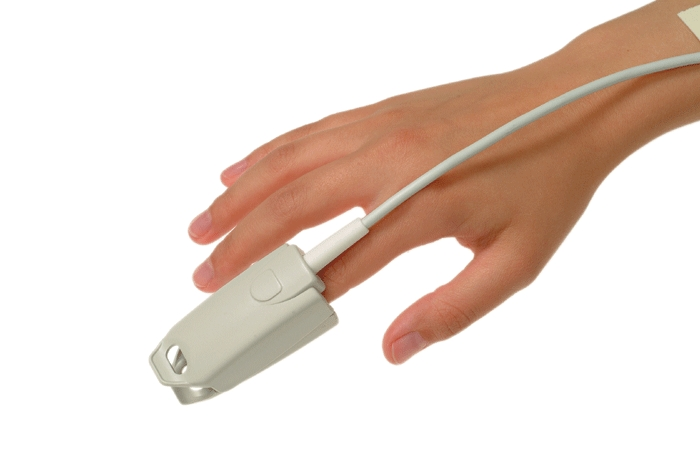
\includegraphics[scale = 0.45]{graphic/sensor}}
	\caption{Sonda pomiarowa pulsoksymetru do badania metodą transluminacji}
	~\\
	(źródło: http://www.covidien.com)
	\label{rys:Sonda}
\end{figure}

\section{Konwerter prąd - napięcie}
\label{sec:LedSterownik}

Celem konwertera jest zamiana sygnału prądowego płynącego ze źródła w~postaci fotodiody na znacznie wygodniejszy z~punktu widzenia dalszej analizy sygnał napięciowy. Uzyskany sygnał w~postaci napięcia 
zmiennego jest poddawany dalszej filtracji i~wzmocnieniu. 
Układ wzmacniacza transimpedancyjnego TIA (ang.~Transimpedance Amplifier) charakteryzuje się bardzo małą rezystancją wejściową. Może on współpracować tylko ze źródłami prądowymi (o dużej rezystancji wewnętrznej), 
ponieważ jego wejście stanowi masę pozorną. 
Wartość prądu wejściowego $I$ nie zależy wówczas od parametrów układu konwertera, ale od źródła sygnału wejściowego~\cite{Rako}. Rysunek~(\ref{rys:IU}) przedstawia schemat konwertera $I/V$.
\begin{figure}[ht]
	\centerline{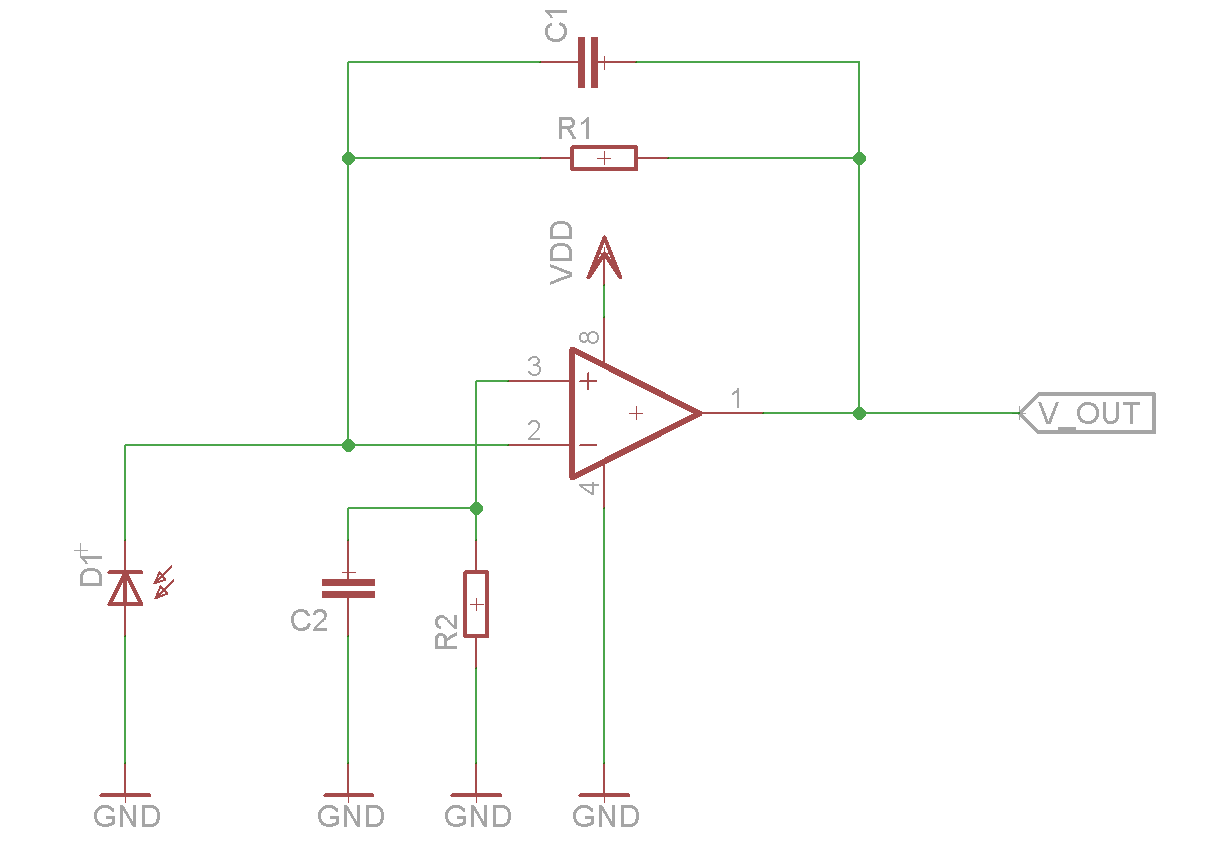
\includegraphics[scale = 0.42]{graphic/IU}}
	\caption{Schemat ideowy konwertera prąd - napięcie na bazie wzmacniacza operacyjnego}
	~\\
	(źródło: Schemat PCB)
	\label{rys:IU}
\end{figure}

Wzmacniacz operacyjny objęty jest pętlą ujemnego sprzężenia zwrotnego, której skutkiem jest istnienie masy pozornej pomiędzy wejściem odwracającym a~wejściem nieodwracającym wzmacniacza. 
Sprzężenie zwrotne realizowane jest za pośrednictwem rezystancji $R_{1}$. Wartość napięcia wyjściowego jest wprost proporcjonalna do prądu wejściowego, a~współczynnik proporcjonalności stanowi rezystancja $R_{1}$.
\begin{equation}
\label{equ:IU}
	V_{OUT} = I_{IN}R_{1}	
\end{equation}

Projektując konwerter prąd - napięcie, autor pracy dużą uwagę skupił na doborze odpowiedniego wzmacniacza operacyjnego o~niskich wejściowych prądach polaryzujących, które sumują się z~sygnałem użytecznym. 
Im mniejsze wartości prądów polaryzujących, tym mniejszy jest błąd przesunięcia napięcia wyjściowego. W~projekcie zastosowano wzmacniacze operacyjne MAXIM MAX4489 o~wejściowych prądach polaryzujących z~przedziału 
1~-~150~pA.

Rozróżnia się dwie metody łączenia źródła fotoprądu w~postaci fotodiody z~układem wzmacniacza transimpedancyjnego. Ze względu na rodzaj odbieranego sygnału należy dokonać wyboru pomiędzy szybkością 
odpowiedzi układu a~precyzją sygnału wyjściowego. Dobór odpowiedniej konfiguracji pracy fotodiody uwarunkowany jest istnieniem pojemności złączowej diody pracującej w~trybie polaryzacji wstecznej~\cite{Rako}. 
Model zastępczy fotodiody półprzewodnikowej przedstawiono na rysunku~\ref{rys:modelPIN}. 

\begin{figure}[ht]
	\centerline{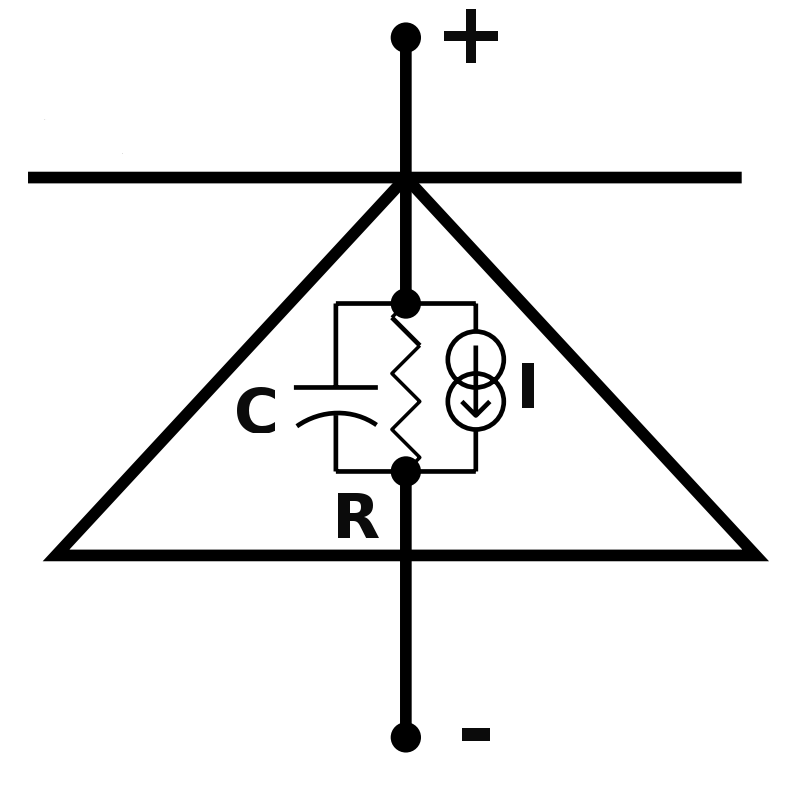
\includegraphics[scale = 0.22]{graphic/modelPIN}}
	\caption{Model fotodiody pracującej w~trybie rewersyjnym}
	~\\
	(źródło: na podstawie \cite{Rako})
	\label{rys:modelPIN}
\end{figure}

Cechą pojemności $C$ złącza P-N jest zmiana jej wartości pod wpływem przyłożonego napięcia rewersyjnego. Wraz ze wzrostem napięcia w~kierunku zaporowym rozszerza się warstwa zubożona stanowiąca dielektryk
kondensatora. Zwiększająca się grubość obszaru zubożonego powoduje zmniejszenie pojemności fotodiody, zmniejszając tym samym czas odpowiedzi fotodiody na impuls promieniowania. Równoległy symbol 
rezystancji $R$ w~modelu symbolizuje prąd ciemny, którego wartość zwiększa się wraz ze wzrostem napięcia na fotodiodzie~\cite{Rako}. 

Ze względu na istnienie powyższych elementów modelu fotodiody rozróżniono fotowoltaiczny i~fotokonduktancyjny tryb pracy~(rys.~\ref{rys:photocond}).
\begin{figure}[ht]
	\centerline{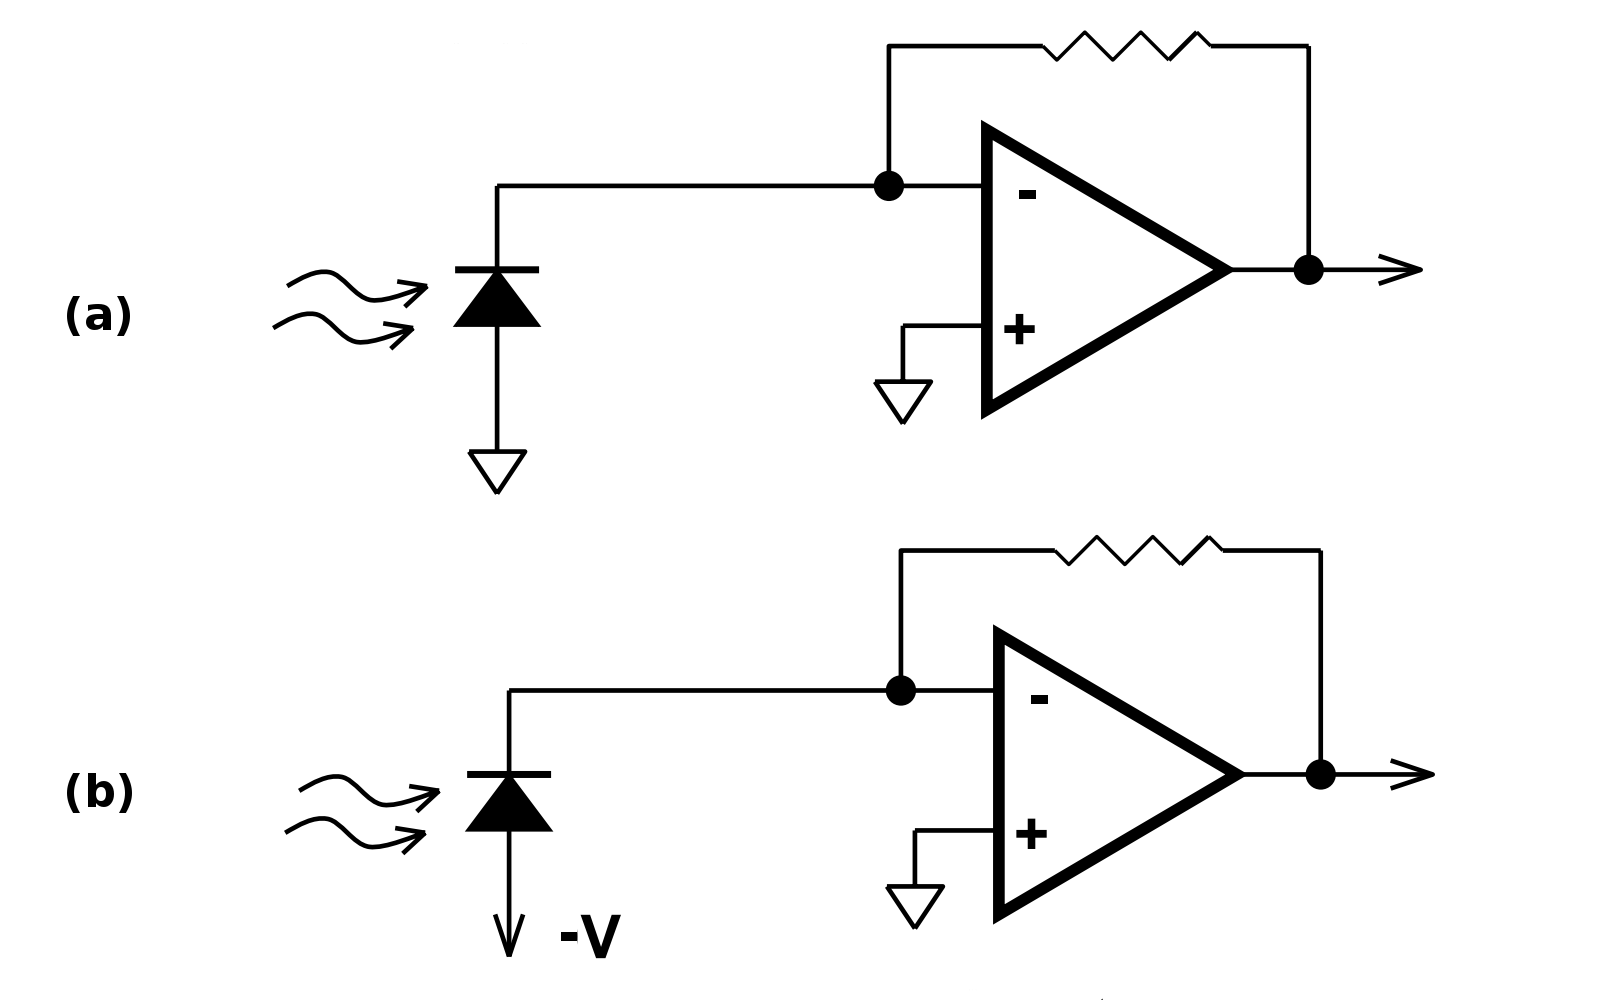
\includegraphics[scale = 0.2]{graphic/photocond}}
	\caption{Tryby pracy fotodiody ze wzmacniaczem transimpedancyjnym: (a) tryb fotowoltaiczny, (b) tryb fotokonduktancyjny}
	~\\
	(źródło: na podstawie \cite{Rako})
	\label{rys:photocond}
\end{figure}

\noindent W~trybie fotowoltaicznym napięcie rewersyjne diody stanowi różnica potencjałów pomiędzy wejściem odwracającym wzmacniacza a~potencjałem masy układu. W~konfiguracji wzmacniacza objętego pętlą ujemnego 
sprzężenia zwrotnego na wejściu odwracającym istnieje masa pozorna. Zatem napięcie rewersyjne diody jest równe wejściowemu napięciu niezrównoważenia. Napięcie to zależy od modelu wzmacniacza operacyjnego 
oraz konkretnego egzemplarza~\cite{Gorecki:2004}.

\noindent Tryb pracy fotowoltaicznej cechuje pomijalnie mała wartość prądu ciemnego rzędu $\mu$A oraz niski poziom szumów, co jest decydujące podczas precyzyjnej detekcji małych sygnałów. W~przypadku trybu fotokonduktancyjnego 
mała pojemność złączowa diody umożliwia pracę z~szybkimi sygnałami o~stromych zboczach~\cite{Rako}. 
W~niniejszym projekcie zastosowano wariant pracy fotowoltaicznej ze względu na detekcję wolnozmiennego sygnału tętna o~niewielkiej amplitudzie.


\subsubsection{Kompensacja częstotliwościowa konwertera $I/V$ }
\label{subsubsec:kompensacja}

Konwerter prąd - napięcie z~rezystorem w~pętli ujemnego sprzężenia zwrotnego jest najprostszą realizacją wzmacniacza transimpedancyjnego (TIA). Pomimo prostoty układu, w~celu zapewnienia poprawnej
pracy wzmacniacza należy dokonać wyboru pomiędzy parametrami, takimi jak poziom szumów, napięcie offsetu, pasmo przenoszenia oraz stabilność. Stabilność głównie jest parametrem kluczowym podczas 
konwersji~\cite{Bhat:2012}.
Układ wzmacniacza transimpedancyjnego, z~pętlą ujemnego sprzężenia zwrotnego podatny jest na oscylacje napięcia wyjściowego. Podatność układu konwertera $I/V$ wynika z~istnienia pojemności
złączowej fotodiody pracującej w~stanie rewersyjnym. W~celu uniknięcia niepożądanych zakłóceń sygnału wyjściowego, układ wzmacniacza kompensowany jest poprzez zastosowanie dodatkowej pojemności $C_{1}$
bocznikującej rezystancję pętli sprzężenia~\cite{Rako}.


\section{Układ próbkująco - pamiętający (Sample and Hold)}
\label{sec:SampleHold}

Multipleksowane sygnały pochodzące od dwóch niezależnych źródeł promieniowania poddawane są detekcji na wspólnym elemencie detekcyjnym oraz wspólnym konwerterze prąd - napięcie. Każdy z~sygnałów jest następnie osobno filtrowany, 
wzmacniany oraz ostatecznie próbkowany w~przetworniku analogowo - cyfrowym. W~związku z~zastosowaniem pojedynczego układu wzmacniacza transimpedancyjnego, niezbędną czynnością okazuje się ponowne
rozdzielenie obu multipleksowanych sygnałów. 
Powyższe wymagania spełnia układ próbkująco - pamiętający, podtrzymujący spróbkowany poziom napięcia na wyjściu konwertera $I/V$~(rys.~\ref{rys:SampleHold}). 

\begin{figure}[ht]
	\centerline{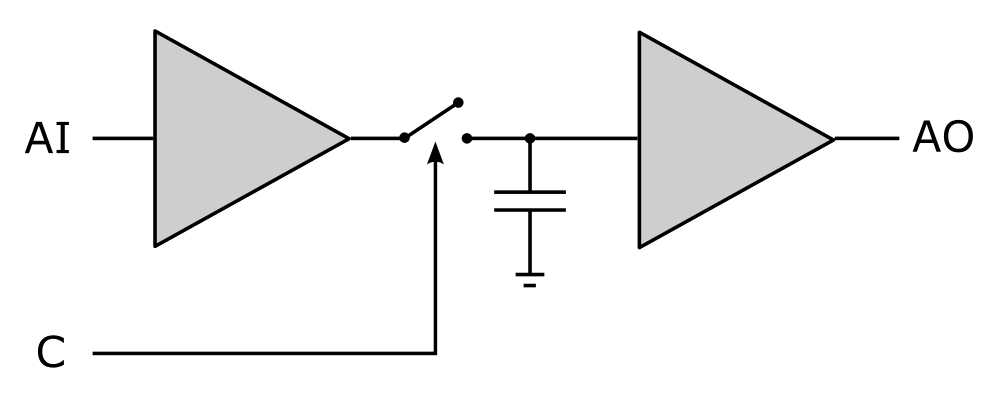
\includegraphics[scale = 0.3]{graphic/SampleHold}}
	\caption{Układ próbkująco~-~pamiętający podtrzymujący napięcie zatrzaśnięte w~chwili próbkowania}
	~\\
	(źródło: http://www.interfacebus.com)
	\label{rys:SampleHold}
\end{figure}

Bufory układu zrealizowano przy pomocy wzmacniacza operacyjnego z~pętlą sprzężenia zwrotnego w~konfiguracji wtórnika napięcia. W~roli elementu kluczującego zastosowano klucz analogowy w~postaci układu scalonego
CMOS 4066. Układ kluczujący zbudowany w~technice CMOS umożliwia przełączanie sygnałów analogowych zbliżonych poziomem zarówno do dodatniej, jak i~ujemnej szyny zasilania~(rys.~\ref{rys:4066}).
\begin{figure}[ht]
	\centerline{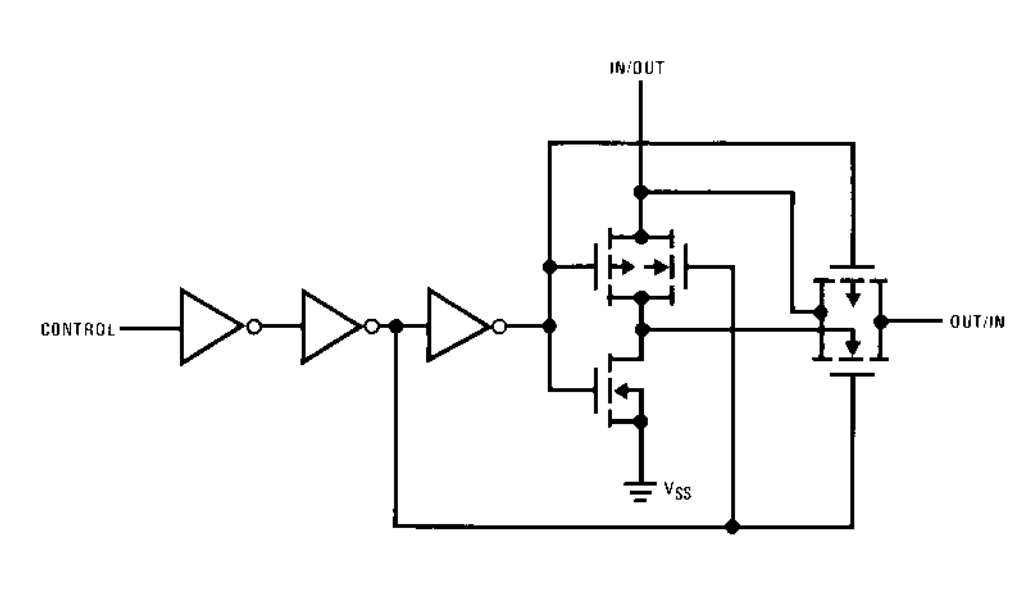
\includegraphics[scale = 0.4]{graphic/4066}}
	\caption{Schemat klucza analogowego układu scalonego CMOS 4066}
	~\\
	(źródło: na podstawie\cite{4066})
	\label{rys:4066}
\end{figure}

Podanie wysokiego stanu logicznego na wejście sterujące klucza analogowego powoduje ładowanie pojemności podtrzymującej do napięcia wejściowego. Zadaniem kondensatora jest podtrzymanie poziomu napięcia
w czasie, gdy klucz jest wyłączony. W~roli bufora napięcia na kondensatorze zastosowano układ wtórnika napięcia o~wysokoimpedancyjnych wejściach nie stanowiących znaczącego obciążenia dla pojemności. 
Nieodłącznym efektem próbkowania sygnałów analogowych jest powstawanie charakterystycznego szumu w~postaci przebiegu schodkowego, związanego ze skończoną wartością częstotliwości sygnału 
kluczującego~(rys.~\ref{rys:samples}).  

\begin{figure}[ht]
	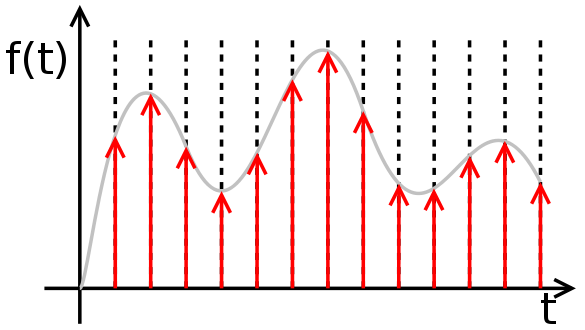
\includegraphics[scale = 0.35]{graphic/sample}
	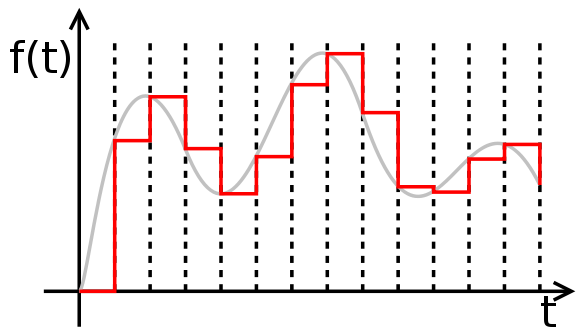
\includegraphics[scale = 0.35]{graphic/sample_hold}
	\caption{Zasada działania układu próbkująco~-~pamiętającego. Charakterystyczny przebieg schodkowy będący efektem próbkowania sygnału analogowego}
	~\\
	(źródło: na podstawie\cite{4066})
	\label{rys:samples}
\end{figure}

W~celu zminimalizowania wpływu szumu próbkowania na dalszy proces analizy sygnału zastosowano wielokrotne zwiększenie częstotliwości próbkowania w~stosunku do częstotliwości sygnału $PPG$, zwane nadpróbkowaniem. 
W~efekcie uzyskuje się przesunięcie widma szumu próbkowania w~kierunku wyższych częstotliwości, co znacznie ułatwia filtrowanie szumu bez degradacji sygnału użytecznego.

\section{Układ filtrujący w~konfiguracji Sallen-Key}
\label{sec:SallenKey}

Szum będący efektem demultipleksacji sygnału w~układzie próbkująco~-~pamiętającym oraz pozostałe szumy generowane przez otoczenie obiektu badanego, w~tym również wpływ zakłóceń elektromagnetycznych oraz oświetlenia 
zewnętrznego, znacząco zniekształcają sygnał uzyskany w~fotodetektorze~(rys.~\ref{rys:filtr1}). Wszystkie źródła zakłóceń generują szumy o~częstotliwościach wyższych od sygnału $PPG$. Najpoważniejsze zakłócenia 
o~częstotliwości 50~Hz generowane są przez sieć energetyczną i~oświetlenie w~postaci żarówek.
\begin{figure}[!ht]
	\centerline{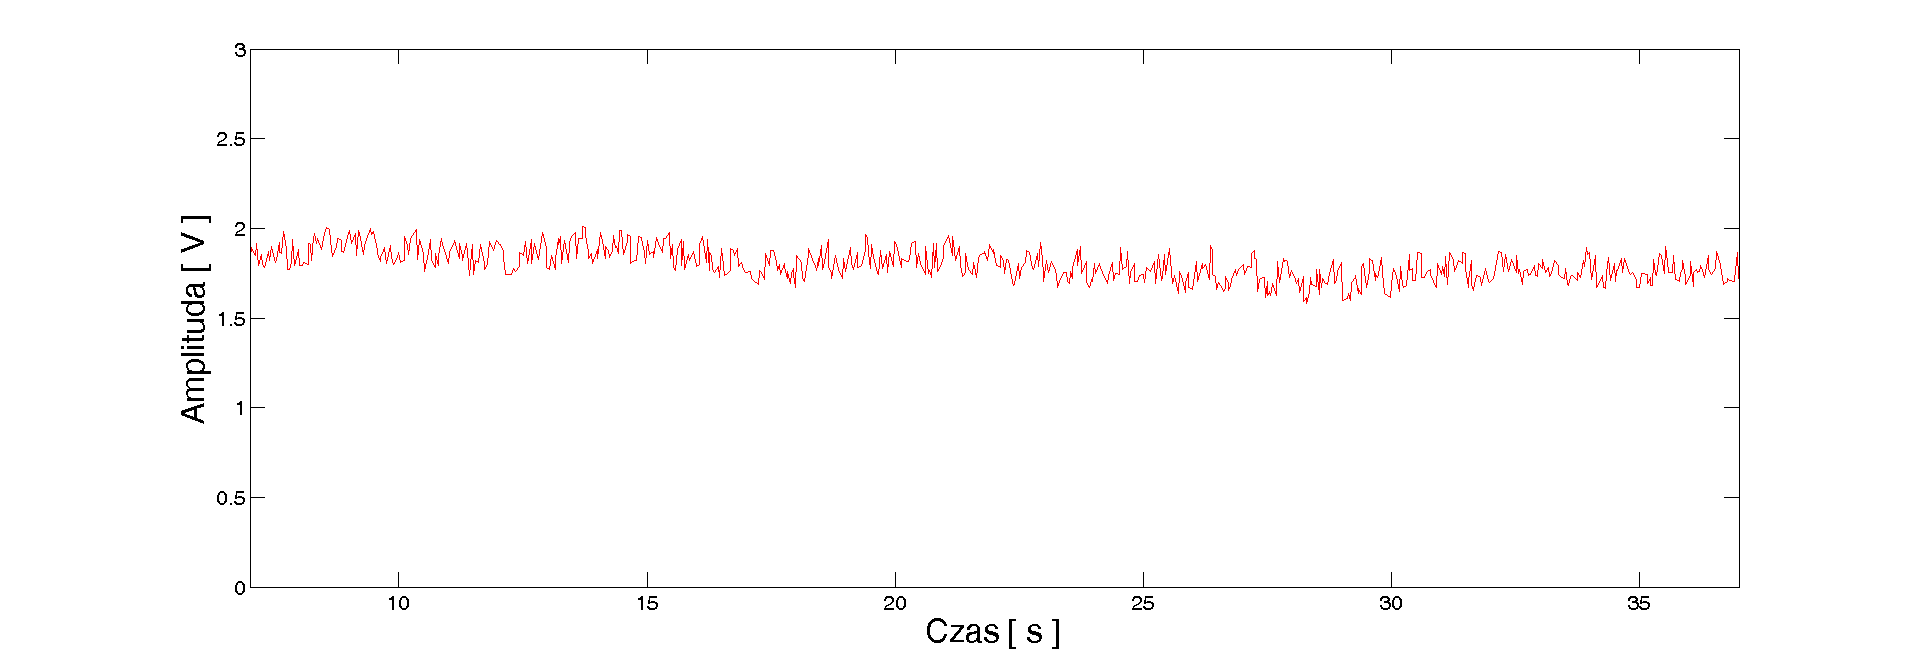
\includegraphics[scale = 0.39]{graphic/filtr1}}
	\caption{Demultipleksowany sygnał diody czerwonej na wyjściu układu próbkująco~-~pamiętającego}
	\label{rys:filtr1}
\end{figure}

Eliminacja szumów  wymaga zastosowania filtru dolnoprzepustowego skutecznie blokującego wszelkie zakłócenia spoza zakresu częstotliwości sygnału użytecznego.
Bliskie sąsiedztwo widma krzywej pletyzmograficznej oraz zakłóceń sieci energetycznej narzuca konieczność stosowania filtrów o~stromych zboczach i~dużej
wartości tłumienia w~pasmie zaporowym. 
Na bazie przeprowadzonych prób i~doświadczeń autor pracy określił wymaganą wartość tłumienia w~paśmie zaporowym na poziomie 50~dB oraz IV rząd filtru. W~celu 
realizacji układu filtru dolnoprzepustowego spełniającego powyższe wymagania zastosowano układ o~topologii Sallen~-~Key~(rys.~\ref{rys:sallenKey}). 
\begin{figure}[!ht]
	\centerline{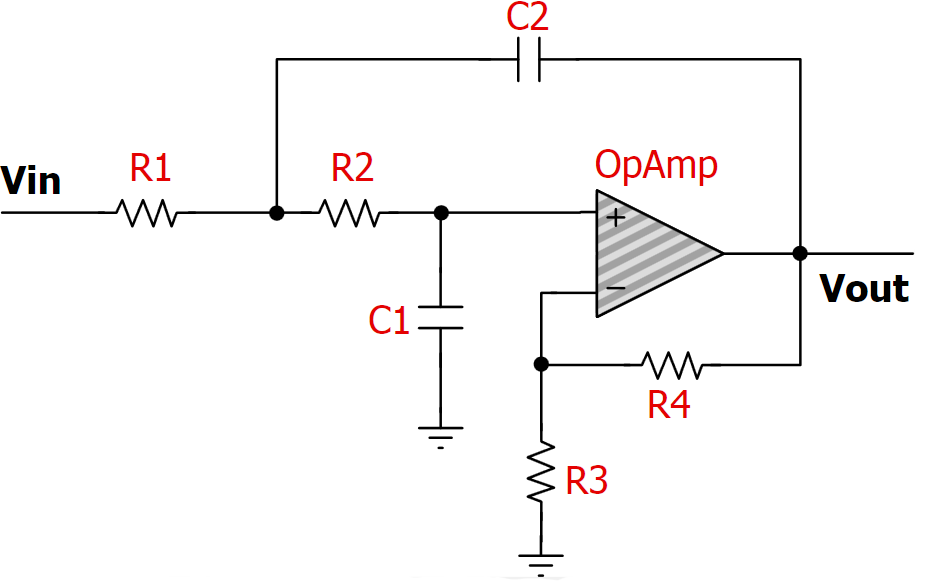
\includegraphics[scale = 0.43]{graphic/sallenKey}}
	\caption{Układ filtru aktywnego o~topologii Sallen~-~Key}
	~\\
	(źródło: na podstawie www.ti.com)
	\label{rys:sallenKey}
\end{figure}

Cechą charakterystyczną zastosowanej konfiguracji jest możliwość implementacji filtrów II rzędu o~różnych charakterystykach przy użyciu pojedynczego wzmacniacza operacyjnego. Filtr IV rzędu uzyskano poprzez 
szeregowe połączenie dwóch segmentów II rzędu. 

Decydujący z~punktu widzenia odpowiedzi filtru na sygnał wejściowy okazał się wybór odpowiedniej charakterystyki amplitudowej. W~fazie projektowania filtru dolnoprzepustowego rozpatrzono charakterystyki 
dolnoprzepustowe Czebyszewa, Butterwortha oraz Bessela. Oceniając odpowiedź układu filtru aktywnego na sygnał analogowy zawierający przebieg fali tętna, parametrem decydującym okazała się podatność poszczególnych 
rodzajów filtru na oscylacje sygnałów wyjściowych (dzwonienie).
Najmniejsze oscylacje zaobserwowano w~filtrach o~charakterystyce Bessela w~przeciwieństwie do układu o~charakterystyce Czebyszewa. Filtr Czebyszewa oraz Butterwortha wykazują znacznie większe nachylenie zboczy 
niż filtr Bessela jednak fakt występowania oscylacji sygnału wyjściowego skutecznie eliminuje możliwość zastosowania filtrów o~charakterystykach tego typu w~układzie pulsoksymetru.
W~układzie pomiarowym zastosowano filtr dolnoprzepustowy o~charakterystyce Bessela w~konfiguracji Sallen~-~Key. Wyznaczenie wartości odpowiednich elementów $R$ i~$C$ dokonano przy użyciu dedykowanego 
oprogramowania FilterPro firmy Texas Instruments~\cite{TI}.\\

Wartości szukanych elementów filtru typu Sallen~-~Key zostały wyznaczone dla następujących parametrów:
\begin{itemize}
	\item Charakterystyka filtru - Bessela
	\item Częstotliwość graniczna dolna - 10~Hz
	\item Częstotliwość graniczna górna - 35~Hz
	\item Maksymalne zafalowania w~paśmie przepustowym - 1~dB
	\item Wartość tłumienia w~paśmie zaporowym - 50~dB
\end{itemize}
\noindent Raport z~symulacji oraz wartości elementów $R$, $C$ zawarto w~dodatku A.\\

Rezultatem filtracji sygnału wyjściowego układu próbkująco~-~pamiętającego jest przebieg na rysunku~\ref{rys:filtr2}.
\begin{figure}[!ht]
	\centerline{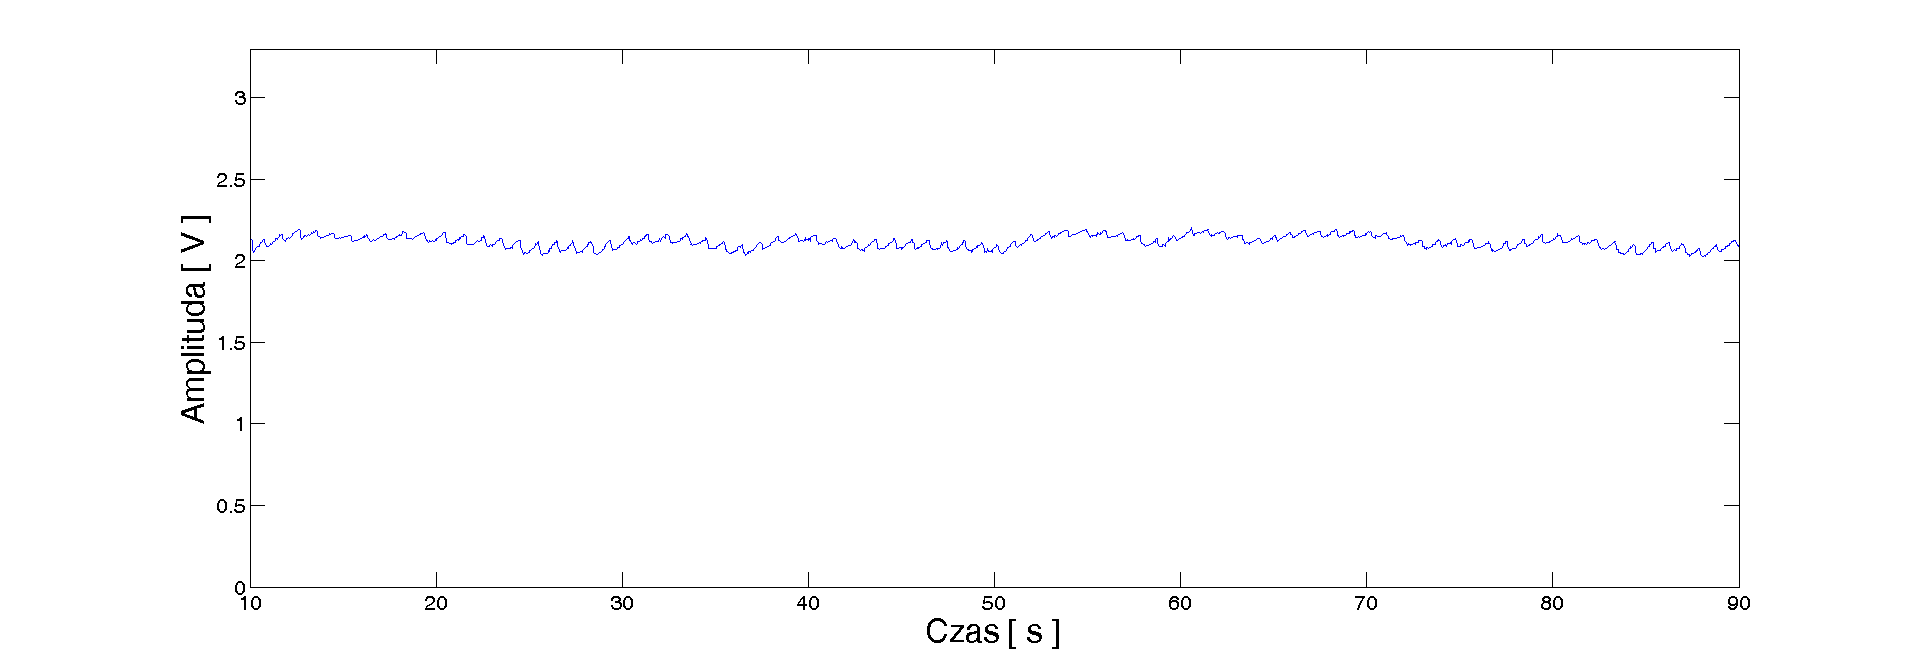
\includegraphics[scale = 0.38]{graphic/filtr2}}
	\caption{Demultipleksowany sygnał diody czerwonej na wyjściu zaprojektowanego filtru dolnoprzepustowego}
	\label{rys:filtr2}
\end{figure}

\subsubsection{Autoregulacja toru pomiarowego}
\label{sec:PID}

Przebieg uzyskany poprzez odfiltrowanie sygnału detektora składa się ze składowej stałej, wolnozmiennego przebiegu krwi żylnej oraz niewielkiego 
przebiegu tętna~(rys.~\ref{rys:calib1}). 
\begin{figure}[ht]
	\centerline{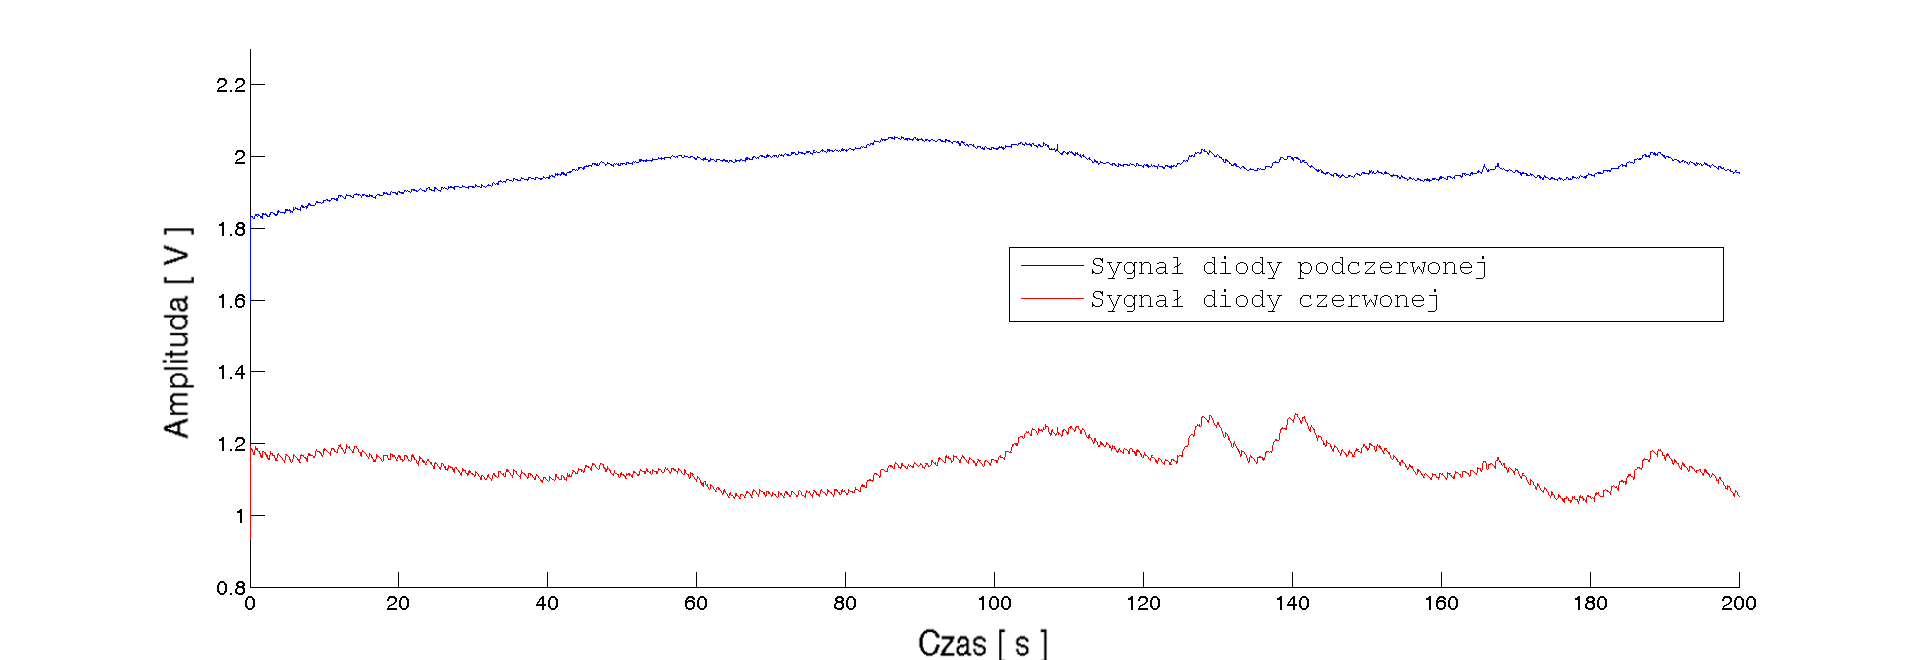
\includegraphics[scale = 0.38]{graphic/calib1}}
	\caption{Sygnał fotodetektora dla dwóch różnych długości fali. Widoczny charakterystyczny sygnał krzywej pletyzmograficznej}
	\label{rys:calib1}
\end{figure}

Wartość składowej DC silnie zależy od grubości, pigmentacji oraz struktury badanego obiektu. W~celu zagwarantowania poprawnej pracy układu 
pomiarowego z~obiektami o~różnych parametrach i~właściwościach, zaproponowano układ autoregulacji toru w~postaci regulatora PID. Pętla 
regulacji obejmuje sterownik źródła promieniowania oraz układ detekcji i~filtrowania sygnału. Układ regulacji kompensuje różnice w~intensywności 
promieniowania diod LED oraz nierównomierność charakterystyki czułości fotodiody. Regulacji podlega wartość składowej stałej sygnału detektora. 

Czas ustalania wartości zadanej zależny jest od współczynników odpowiednich członów regulatora PID. Autor projektu dokonał serii
prób doświadczalnych przy pomocy metod Zieglera~-~Nicholsa, których celem był dobór odpowiednich parametrów regulatora. Zastosowanie metod doświadczalnych,
uwarunkowane zostało brakiem znajomości transmitancji toru pomiarowego. 
Współczynniki regulatora PID wyznaczone na podstawie przyjętych metod nie spełniły założonych wymagań. Rezultaty empirycznej metody doboru parametrów
polegającej na iteracyjnej korekcie współczynników przedstawia rysunek~(rys.~\ref{rys:polka}).
\begin{figure}[ht]
	\centerline{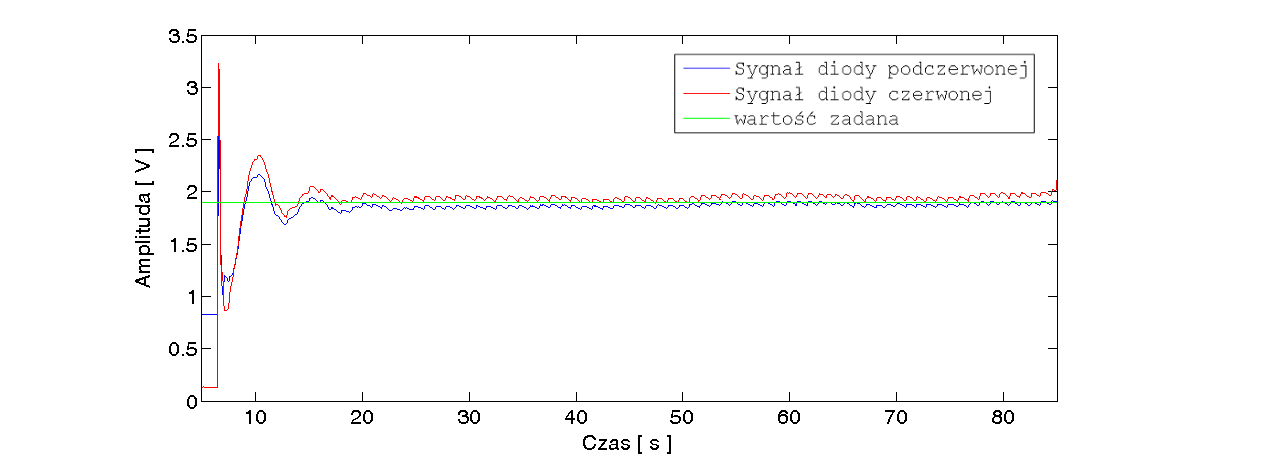
\includegraphics[scale = 0.58]{graphic/pid2}}
	\caption{Przebieg procesu regulacji sygnałów dwóch źródeł promieniowania}
	\label{rys:pid2}
\end{figure}

Alternatywą dla regulatora PID w~układzie pulsoksymetru jest ustalanie wartości zadanej przez stopniową, liniową regulację prądu zasilającego diody 
LED~(rys.~\ref{rys:polka}).
\begin{figure}[!ht]
	\centerline{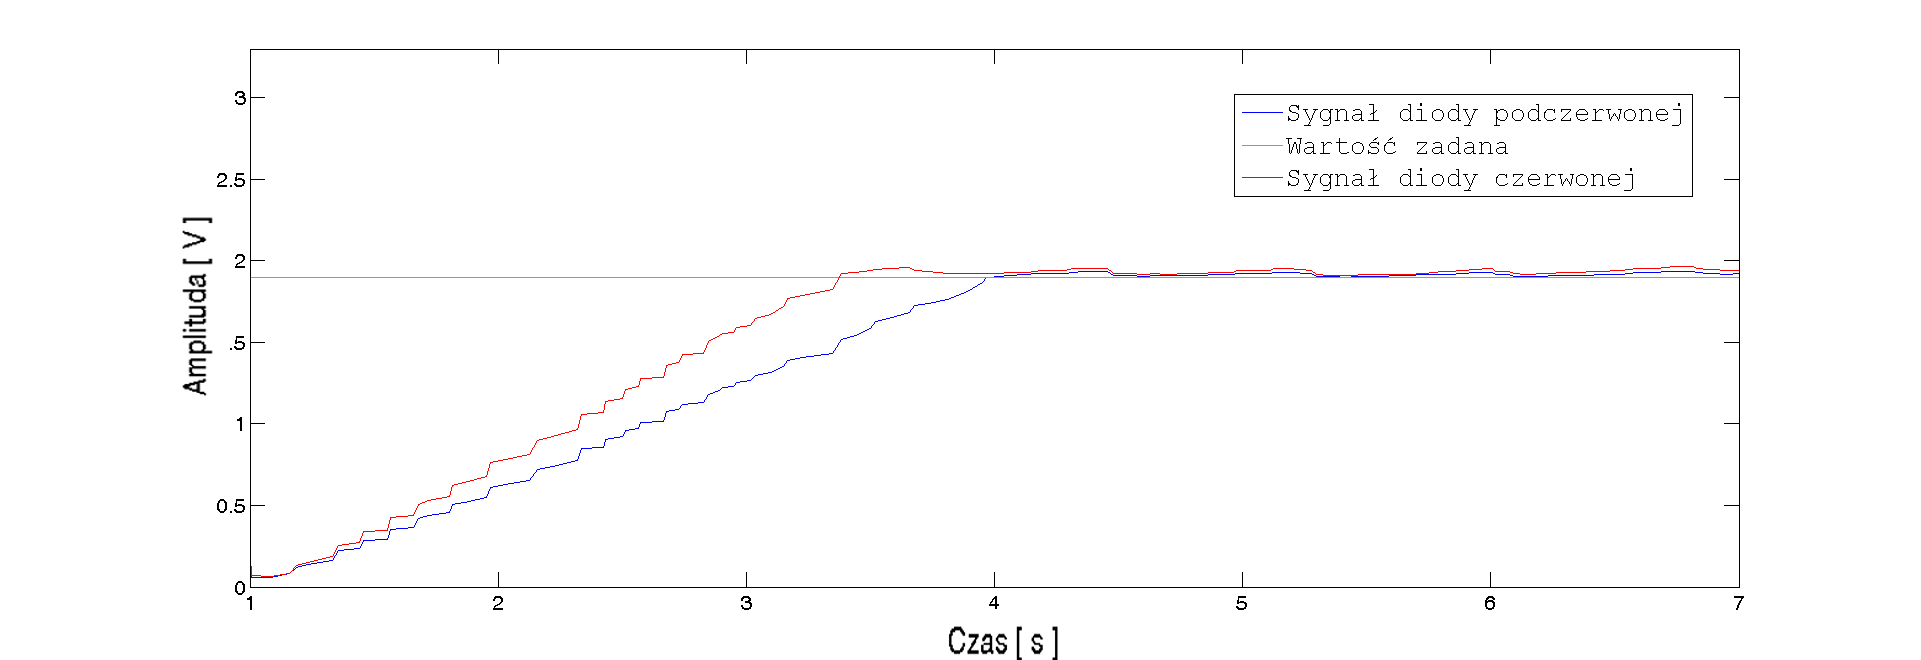
\includegraphics[scale = 0.38]{graphic/polka}}
	\caption{Proces liniowej regulacji intensywności promieniowania diod LED}
	\label{rys:polka}
\end{figure}

\noindent Czas ustalania wartości zadanej jest znacząco krótszy w~stosunku do czasu ustalania przedstawionego regulatora PID. Regulacja poziomu sygnałów
wyjściowych ma na celu utrzymanie ich na stałym poziomie, co jest niezbędne podczas pomiarów saturacji krwi~(rys.~\ref{rys:polka2}).
\begin{figure}[!ht]
	\centerline{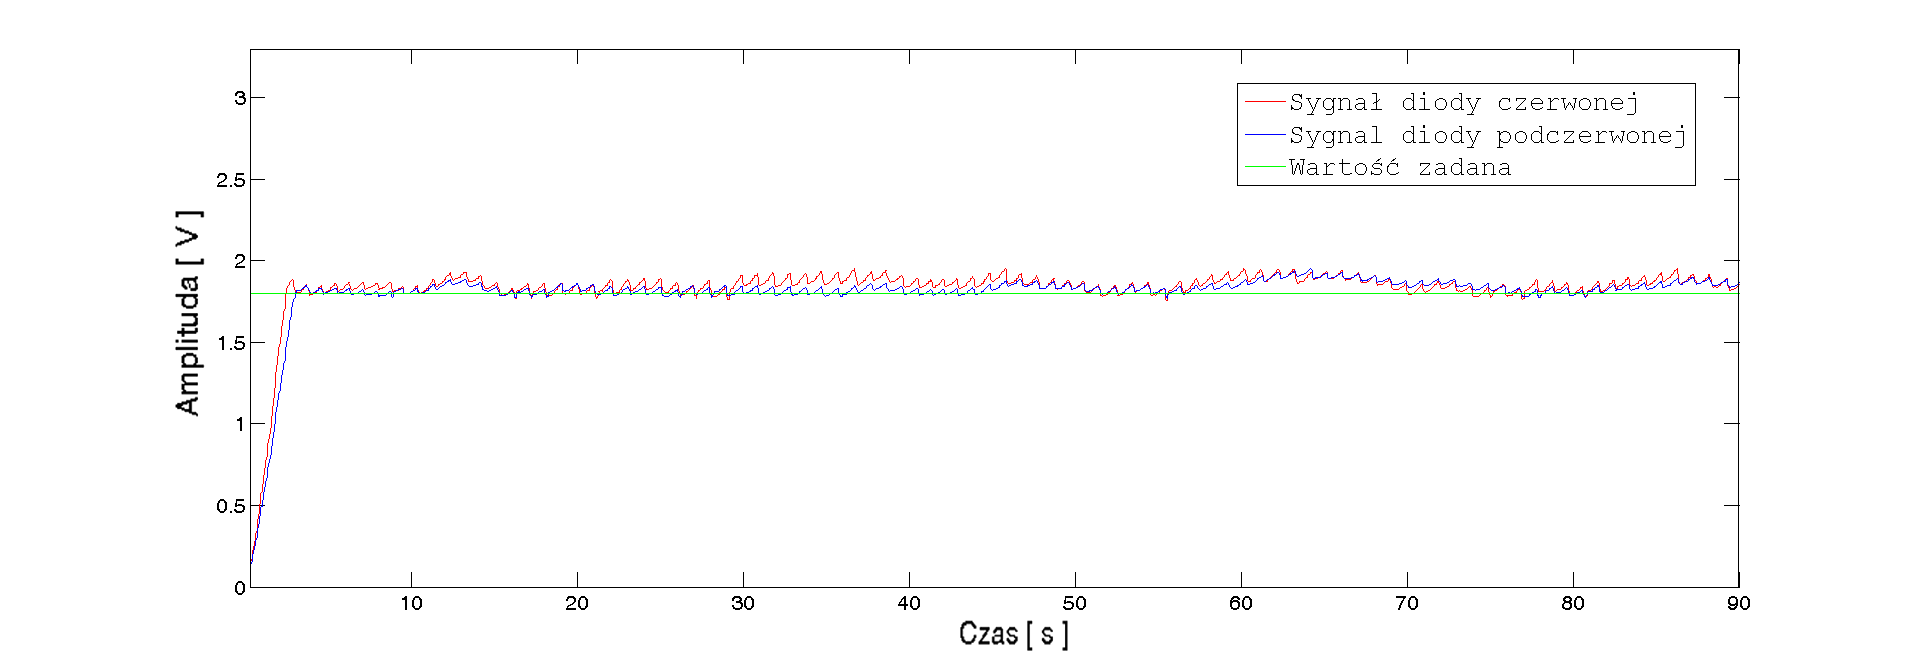
\includegraphics[scale = 0.40]{graphic/polka2}}
	\caption{Proces utrzymywania stałego poziomu sygnałów diod LED}
	\label{rys:polka2}
\end{figure}\\

\section{Wzmacniacz o~regulowanym wzmocnieniu}
\label{sec:PGA}

Obniżenie temperatury otoczenia do niższych wartości od strefy komfortu cieplnego skóry uruchamia mechanizmy adaptacyjne regulacji cieplnej 
ustroju~\cite{SzGa11}. W~pierwszej fazie krótkotrwałego działania zimna skóra jest blada. Skurcz naczyń krwionośnych skóry i~tkanki podskórnej 
występujący pod wpływem niskich temperatur, zmniejsza przepływ krwi i~ogranicza w~ten sposób oddawanie ciepła otoczeniu. Obniżona elastyczność 
tętniczych naczyń krwionośnych skutecznie ogranicza możliwość detekcji fali tętna w~postaci krzywej pletyzmograficznej ($PPG$).

Wpływ temperatury badanego obiektu na amplitudę prądu fotodiody wymusza konieczność zastosowania układu dopasowującego sygnał PPG do zakresu
napięć wejściowych przetwornika analogowo~-~cyfrowego~(rys.~\ref{rys:PGA}).  
\begin{figure}[ht]
	\centerline{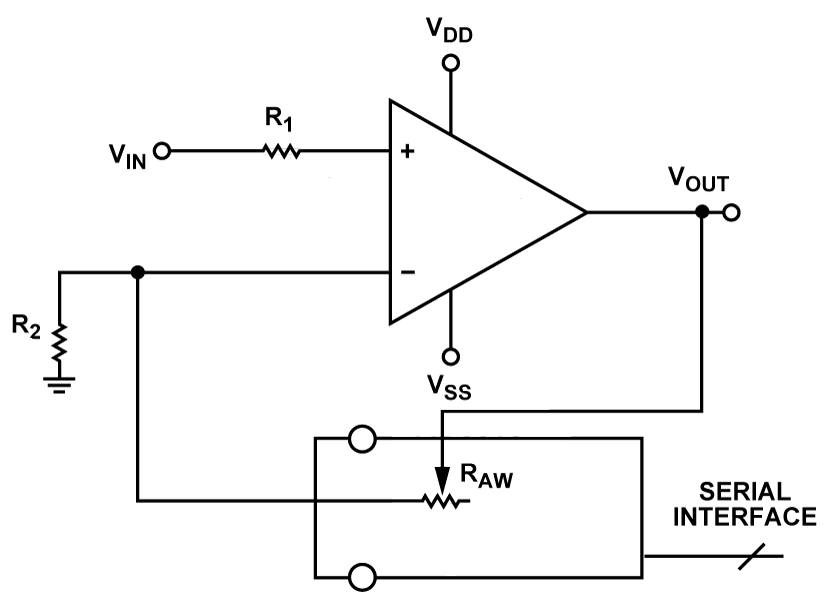
\includegraphics[scale = 0.3]{graphic/PGA}}
	\caption{Wzmacniacz operacyjny pracujący jako układ o~zmiennym wzmocnieniu w~konfiguracji nieodwracającej}
	~\\
	(źródło: www.analog.com)
	\label{rys:PGA}
\end{figure}

Wzmacniacz o~regulowanym wzmocnieniu PGA (ang.~Programmable Gain Amplifier) został zrealizowany na bazie wzmacniacza operacyjnego pracującego 
w~konfiguracji nieodwracającej. Regulacja wzmocnienia odbywa się poprzez zastosowanie przestrajanego potencjometru sterowanego cyfrowo.

Wzmocnienie układu wyraża zależność:
\begin{equation}
\label{equ:AMP}
	k_{u} = 1 + \frac{R_{AW}}{R_{2}} 	
\end{equation}

Praca wzmacniacza z~napięciami wejściowymi w~pobliżu dodatniej szyny zasilania wymusza zastosowanie wzmacniacza operacyjnego o~specjalnej konstrukcji
wejściowego stopnia różnicowego (Rail-to-Rail input). Postawione wymagania spełnia wzmacniacz operacyjny typu OPA340. W~roli potencjometru w~pętli 
ujemnego sprzężenia zwrotnego zastosowano potencjometr cyfrowy Microchip MCP41050 o~rezystancji $50~k\Omega$. Sterowanie nastawami potencjometru odbywa
się za pośrednictwem transmisji szeregowej i~interfejsu SPI (ang. Serial Peripherial Interface).

Rezultat zastosowania układu regulowanego wzmacniacza przedstawiono na przebiegu~\ref{rys:wzm}.
\begin{figure}[!h]
	\centerline{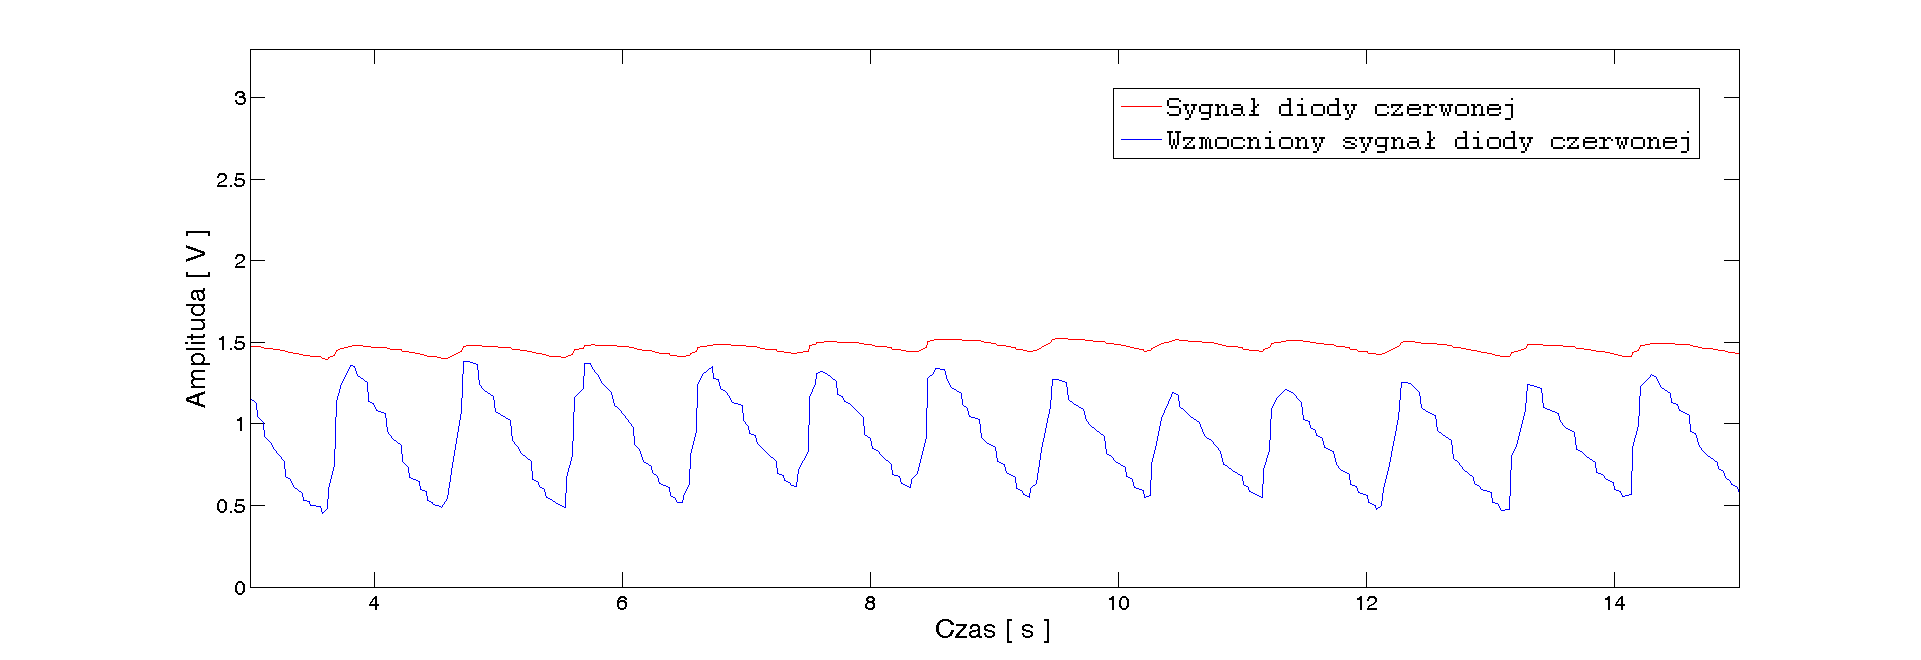
\includegraphics[scale = 0.42]{graphic/wzm}}
	\caption{Przebieg krzywej pletyzmograficznej przed i~po wzmocnieniu}
	\label{rys:wzm}
\end{figure}\\

\section{Mikrokontroler sterujący i~wizualizacja wyników}
\label{sec:ARM}

Rdzeń ARM Cortex M3 wraz z~bogatym zestawem układów peryferyjnych, stanowiący układ mikrokontrolera STM32, odpowiedzialny
jest za kontrolę całego procesu pomiarowego. Podstawowe zadania systemu kontrolnego to generowanie sygnałów kluczujących diody LED, 
sterowanie intensywnością światła, regulacja układu PGA oraz obsługa transmisji szeregowej z~nadrzędnym komputerem PC. 
Obliczanie parametrów życiowych odbywa się w~sposób programowy na podstawie danych uzyskanych z~przetworników analogowo~-~cyfrowych.

Konieczność równoczesnej kontroli wielu parametrów procesu pomiarowego wymusza zastosowanie systemu operacyjnego czasu
rzeczywistego. Procedury kontrolno~-~sterujące zrealizowane w~formie odrębnych procesów znacznie ułatwiają ewaluację
kodu źródłowego aplikacji i~proces jego zarządzania. W~pracy zastosowano system operacyjny FreeRTOS w~wersji 7.3.0.\\

Przedstawienie wyników pomiaru częstości akcji serca i~saturacji oraz przebiegi krzywej pletyzmograficznej zrealizowano w~formie
prostej aplikacji w~środowisku LabView~(rys.~\ref{rys:GUI}).\\ 
\begin{figure}[ht]
	\centerline{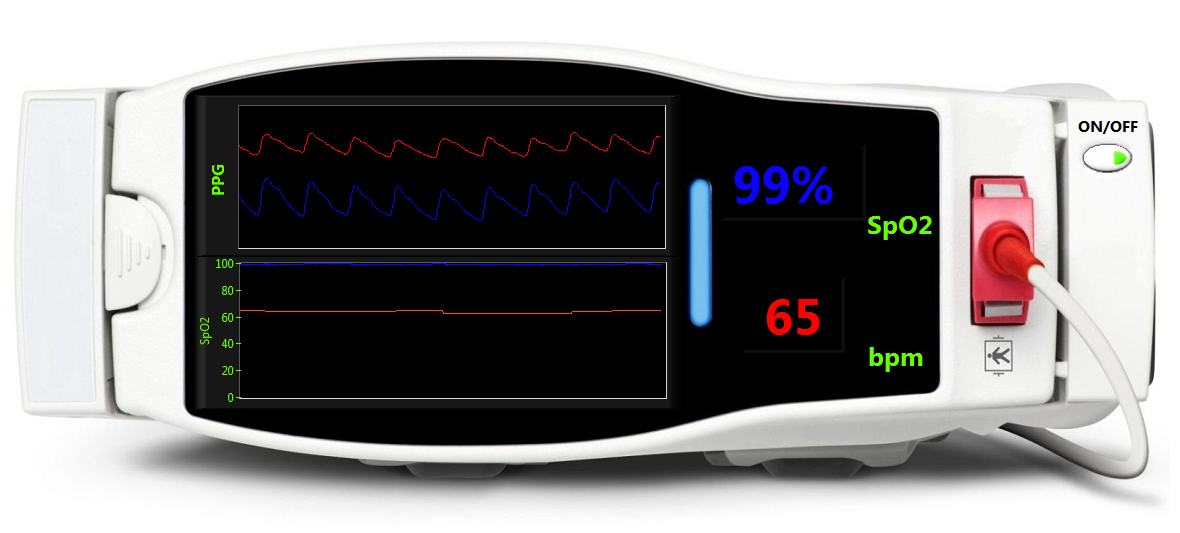
\includegraphics[scale = 0.55]{graphic/GUI}}
	\caption{Panel czołowy pulsoksymetru w~formie wirtualnego przyrządu LabView}
	\label{rys:GUI}
\end{figure}

Komunikacja z~aplikacją odbywa się poprzez szeregową transmisję na porcie USB. Środowisko LabView umożliwia w~łatwy i~przystępny sposób 
rejestrowanie, analizę oraz wizualizację wyników pomiaru. Dodatkowo istnieje możliwość zapisu uzyskanych danych na dysku twardym komputera 
oraz ich poźniejsze wykorzystanie.

Kompletne urządzenie pomiarowe w~formie obwodu drukowanego PCB wraz z~opisem poszczególnych fragmentów projektu przedstawiono poniżej~(rys.~\ref{rys:PCB}).
\begin{figure}[ht]
	\centerline{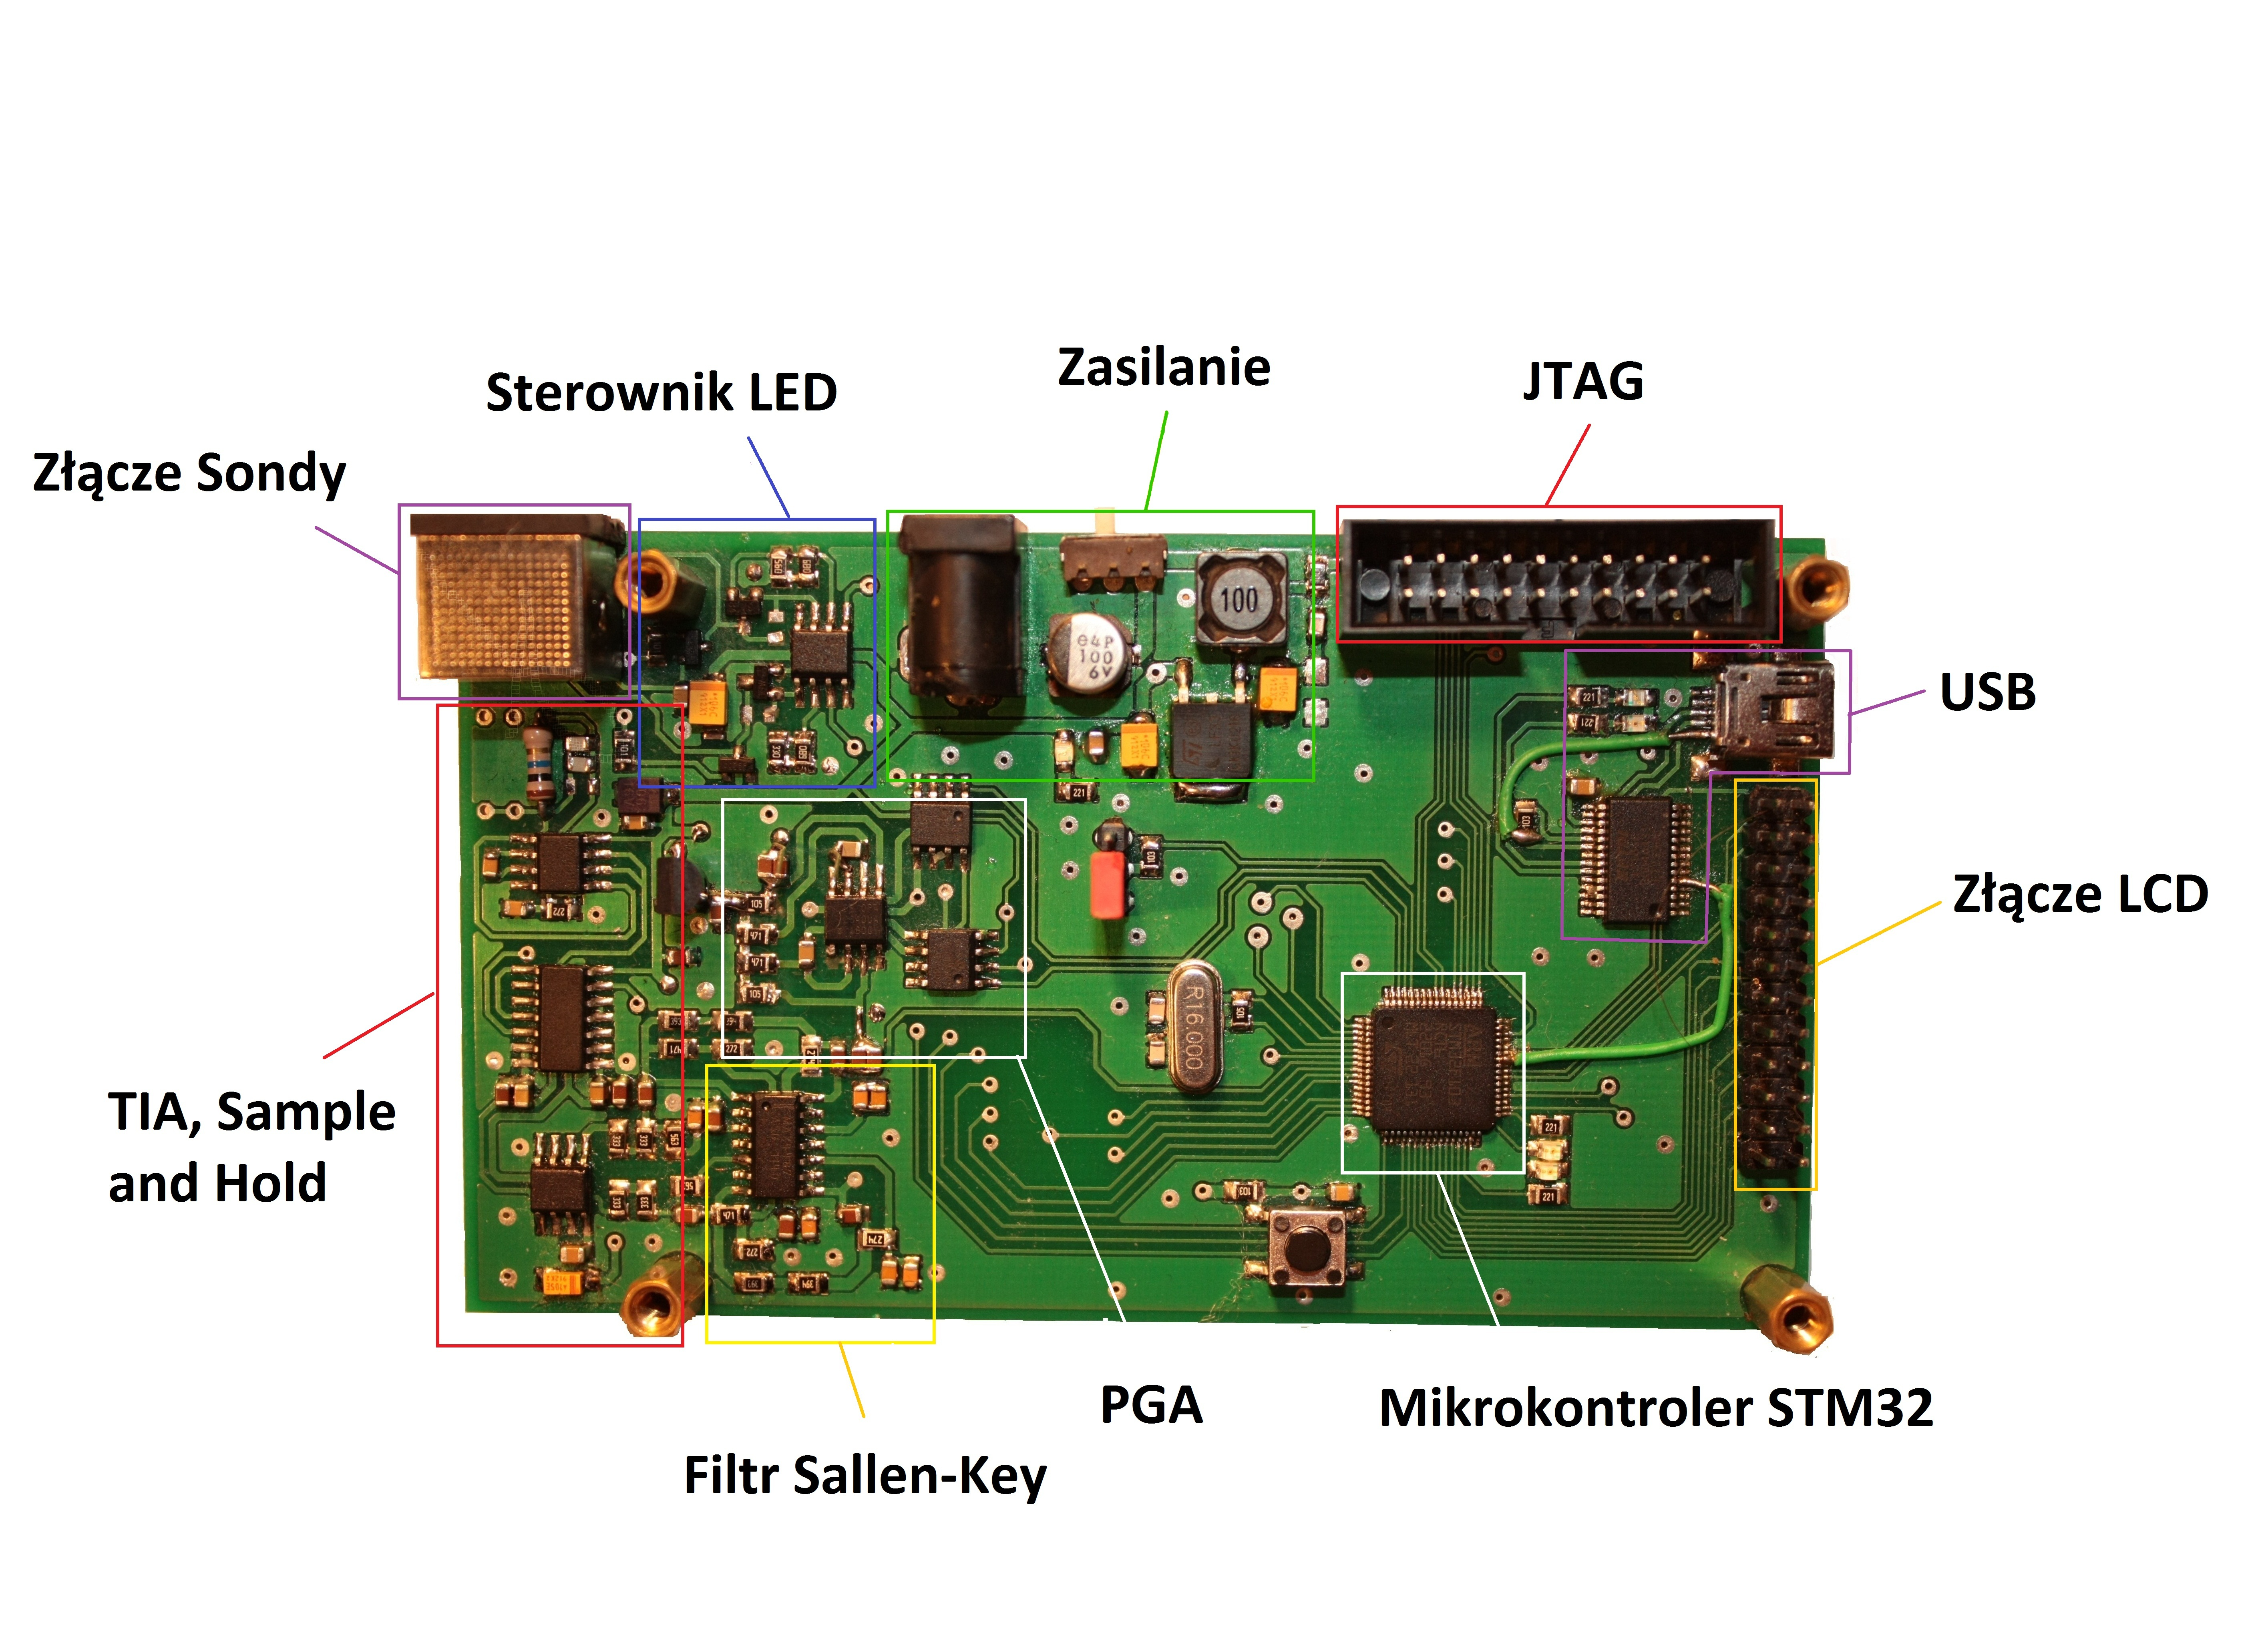
\includegraphics[scale = 0.11]{graphic/PCB}}
	\caption{Widok gotowego urządzenia pomiarowego wraz z~opisem najważniejszych elementow układu}
	\label{rys:PCB}
\end{figure}




